\section{Séance 1 : l'offre et la demande}

\begin{center}
    \begin{tabular}{cc}
        \multicolumn{2}{c}{\includegraphics[width=0.25\textwidth]{images/graph_equilibre.pdf}}\\
        \includegraphics[width=0.25\textwidth]{images/graph_offre_augmente.pdf}&
        \includegraphics[width=0.25\textwidth]{images/graph_demande_augmente.pdf}\\
        L'offre \textcolor[rgb]{1,0,0}{augmente} de façon autonome en \textcolor[rgb]{1,0,0}{O'}&La demande \textcolor[rgb]{1,0,0}{augmente} de façon autonome en \textcolor[rgb]{1,0,0}{D'}\\
        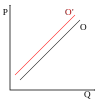
\includegraphics[width=0.25\textwidth]{images/graph_offre_diminue.pdf}&
        \includegraphics[width=0.25\textwidth]{images/graph_demande_diminue.pdf}\\
        L'offre \textcolor[rgb]{1,0,0}{diminue} de façon autonome en \textcolor[rgb]{1,0,0}{O'}&La demande \textcolor[rgb]{1,0,0}{diminue} de façon autonome en \textcolor[rgb]{1,0,0}{D'}
    \end{tabular}
\end{center}

\begin{tabular}{llllll}
    Équation de la demande:    & $D$ & $\equiv$ & $P$ & $=$ & $a - bQ$\\
    Équation de l’offre:       & $O$ & $\equiv$ & $P$ & $=$ & $c + dQ$\\
    Prix à l’équilibre:        &     &          & $O$ & $=$ & $D$
\end{tabular}